
\subsection{Abstract}

In this paper, an algorithm for performing System Identification and inference of the filtering recursion for stochastic non-linear dynamical systems is introduced. Additionally, the algorithm allows for enforcing domain-constraints of the state variable. The algorithm makes use of an approximate inference technique called Variational Inference in conjunction with Deep Neural Networks as the optimization engine. Although general in its nature, the algorithm is evaluated in the context of Non-Intrusive Load Monitoring, the problem of inferring the operational state of individual appliances given aggregate measurements collected in a home.


\subsection{Introduction}
\label{sec:intro}

System Identification and Inference for dynamical systems has a long history~\cite{ljung1998system}. In this paper we consider systems of the following type:
\begin{align*}
z_t \sim p(z_t | z_{t-1}, \Theta) \> \> \> \>x_t \sim p(x_t | z_t, \Theta)
\end{align*}
where $p$ is some distribution known up to parameters $\Theta$, $x$ and $z$ constitutes the observation and unknown latent state respectively. For e.g. linear dynamical systems optimal solutions such as the Kalman filters~\cite{kalman1960contributions} and subspace methods~\cite{van2012subspace} exists. However, when the system dynamics are assumed to be non-linear and stochastic non-optimal techniques such as particle filters in conjunction with Expectation Maximization need to be resorted to. The bottleneck for these approaches is oftentimes the computation of the filtering recursion $p(z_t | x_{1:t},\Theta)$ which for many latent variable models is computationally intractable. 
We propose a novel algorithm in which maximizing the data likelihood $p(x_{1:T}|\Theta)$ is learned jointly with performing inference of the intractable filtering recursion. The algorithm makes use of an approximate statistical inference technique called Variational Inference (VI). VI has recently received increased attention from the Machine Learning community. Recent breakthroughs have improved the applicability~\cite{ranganath2014black}, scalability~\cite{hoffman2013stochastic,kingma2013auto} and accuracy~\cite{rezende2015variational,lange2018factornet} of the technique. See~\cite{zhang2017advances,blei2017variational} for reviews of the approach. 
The algorithm will be showcased in the context of Non-Intrusive Load Monitoring~\cite{hart1992nonintrusive} (NILM) which is the problem of inferring the operational state of appliances within a home given aggregate consumption measurements collected at a single sensing point and was first introduced in the seminal paper by Hart~\cite{hart1992nonintrusive}. The application of VI to NILM is not new~\cite{lange2018varbolt,ng2016scaling}, however, previous approaches relied on the assumption that the system dynamics can be factorized, i.e. these approaches perform inference in a model called Factorial Hidden Markov Model~\cite{ghahramani1996factorial}. Note that NILM is a challenging problem because the latent variable is usually assumed to be binary, i.e. $z_t \in Z = \{0,1\}^C$ where $C$ is the number of components to be inferred. This integrality constraint is challenging for two reasons. First, linearizing approaches like Extended Kalman filters become hard to apply and enumerating the latent domain is computationally intractable because the cardinality of $Z$ grows exponentially with $C$. As we will show later, like VI generalizes Expectation Maximization to latent variable models with intractable posterior, the main contribution of this paper is the generalization of VI to a class of latent variable models with intractable joint distribution. This class constitutes dynamical systems.
%In the next subsection a brief introduction into Variational Inference is given and the problem of intractable joint distributions is presented. After this, a method to tackle intractable joint distributions encountered in dynamical systems is presented followed by variance red

\subsection{Variational Inference}
\label{sec:format}
We begin by deriving Variational Inference from the Expectation Maximization (EM) algorithm. The EM algorithm~\cite{dempster1977maximum} is an algorithm to perform maximum likelihood inference on unknown parameters $\Theta$ in a latent variable model governed by observations $x$ and latent variables $z$, i.e. it maximizes $\sum_z p_\Theta(x,z)$ w.r.t. $\Theta$\footnote{For notational convenience, model parameters are moved to the subscript, i.e. $p(x|\Theta) = p_\Theta(x)$.}. It can be shown that EM performs coordinate ascent on a function $F_1$ known as the Variational Free Energy defined by:
\begin{align*}
F_{1}(\Theta, \tilde{P}) = \mathbb{E}_{\tilde{P}} \log p_\Theta(x,z) - \mathbb{E}_{\tilde{P}} \log \tilde{p}(z)
\end{align*} Specifically, maximizing $F_1$ in the direction of $\tilde{P}$ (the E-step) computes $\tilde{P} = p(z|x)$ whereas the maximization step in the direction of $\Theta$ (the M-step) improves $p(x|\Theta)$~\cite{neal1998view}. Therefore, because the E-step requires computing the posterior, EM is only applicable if computing the posterior $p(z|x)$ is computationally tractable. However, for many latent variable models, computing the posterior is computationally intractable because the denominator of $p(z|x)=\frac{p(z,x)}{\sum_{z\in Z} p(z,x)}$ is oftentimes hard to compute if the support of the latent variable is large. Variational Inference (VI) is a generalization of EM to latent variable models with intractable posterior distributions~\cite{jordan1999introduction}.\\
The main idea behind Variational Inference is the introduction of a tractable auxiliary distribution $Q_\psi$ parameterized by the variational parameters $\psi$. $Q_\psi$ is chosen from a family of distributions such that ideally, there is a $\psi$ such that $q_\psi(z|x) = p_\Theta(z|x)$ and because of recent successes of Neural Networks for non-linear optimization, $Q_\psi$ is often parameterized by Neural Nets. For VI, a function akin to $F_1$ is maximized that substitutes $\tilde{P}$ for the auxiliary but tractable distribution $Q_\psi$.
\begin{align*}
F_{2}(\Theta, \psi) &= \mathbb{E}_{q_\psi(z|x)} \log p_\Theta(x,z) - \mathbb{E}_{q_\psi(z|x)} \log q_\psi(z|x)\\
&=  \log p_\Theta(x) - D_{KL}(q_\psi(z|x) || p_\Theta(z|x))
\end{align*}
Maximizing $F_2$ w.r.t. $\Theta$ optimizes a lower bound of the evidence. This bound is tight if  $q_\psi(z|x)=p_\Theta(z|x)$, i.e. $D_{KL}(q(z|x) || p_\Theta(z|x)) = 0$. Furthermore, maximizing $F_2$ w.r.t. $\psi$ minimizes the KL-divergence, i.e. it tightens the bound. Note that, because of these properties, VI also allows for performing posterior inference. After the optimization procedure, because $Q_\psi$ will be maximally similar to $P_\Theta$, in order to perform posterior inference on the intractable $P_\Theta$, inference is performed on $Q_\psi$ instead. However, note that although Variational Inference generalizes the EM algorithm to latent variable problems with intractable posterior distributions, it still requires the joint distribution $p_\Theta(x,z)$ to be tractable. However, for many latent variable models even the joint distribution might be intractable. One such class of problems constitute temporal models. In this paper, we generalize VI to this class of problems.

\subsection{Intractable Joint}

The class of latent variable models of interest constitute dynamical systems in which the latent state evolves over time according to dynamics adhering to the first-order Markov assumption and the observation is some probabilistic function of the system state. This entails that the joint distribution of the observation and system states can be factored based on $p(x_t | z_t)$ and $p(z_t|z_{t-1})$\footnote{For notational convenice, all dependencies on parameters $\Theta$ and $\psi$ are omitted.}, i.e.:
\begin{align*}
p(x_{1:T}, z_{0:T}) = p(z_0) \prod_{t=1}^T p(x_t | z_t) p(z_t|z_{t-1})
\end{align*}

Let $\alpha_t = \alpha(z_t|x_{1:t})$. For such a model, a lower bound of the chain-rule factorization of the likelihood can be derived as:
\begin{align}
F_{3}(\Theta, \psi, t) &= \mathbb{E}_{q_t} \log p_\Theta(x_t,z_t|x_{1:t-1}) - \mathbb{E}_{q_t} \log q_t \label{f3}\\
&=  \log p_\Theta(x_t|x_{1:t-1}) - D_{KL}(q_t || p_t)
\end{align}


Note that summing $F_3$ over time steps implies that a lower bound of the log-evidence is maximized since:
\begin{align*}
\sum_{t=0}^T F_3(\Theta, \psi, t) = \log p_\Theta(x_{1:T}) - \sum_{t=1}^T D_{KL}(q_t || p_t)
\end{align*}

However, evaluating this bound is intractable for many latent variable models of interest because the joint distribution is intractable as seen below:
\begin{align}
p(x_t,z_t|x_{1:t-1}) = p(x_t|z_t) \sum_{z' \in Z} p(z_t|z') p(z' | x_{1:t-1}) \label{joint}
\end{align}
First, the summation over the latent domain is usually intractable. Second, evaluating equation (\ref{joint}) at time point $t$ requires knowledge of the posterior at time $t-1$ which is intractable.

\subsubsection{Monte Carlo Integration and Importance Sampling}
\label{MC-IS}
In the following, we will show how an unbiased approximation can be obtained that makes use of Monte Carlo Integration in conjunction with Importance Sampling \cite{mcbook}.

Monte Carlo Integration (MC) is a numerical technique to approximate an expectation of the type $\mathbb E_{p(z)} f(z)$ by sampling, i.e. $N$ samples are drawn i.i.d. from $p(z)$ and $\mathbb E_{p(z)} f(z) \approx \frac{1}{N} \sum_{i=1}^N f(z^{(i)})$ with $z^{(i)} \sim p(z)$.

Note that the intractable summation in equation (\ref{joint}) can be written as an expectation of this type, i.e. 
\begin{align}
p(x_t,z_t|x_{1:t-1}) = p(x_t|z_t) \mathbb E_{p_{t-1}} p(z_t|z_{t-1})  \label{joint2}
\end{align}
However, drawing samples from $p(z_{t-1} | x_{1:t-1})$ is not trivial and would require time-consuming advanced samplers. Instead, a technique to change the sampling distribution is being employed called Importance Sampling.

Importance Sampling is usually used as a variance reduction technique. However, in this case, it will be used to ease the computational burden of approximating equation (\ref{joint2}). The general idea is the following: Sampling from $p(z_{t-1} | x_{1:t-1})$ is computationally challenging, however, we have access to a distribution similar to $P$ for which simulating samples is in comparison computationally cheap, namely the auxiliary distribution $Q$. We can rewrite equation (\ref{joint2}) in the following way:
\begin{align}
p(x_t,z_t|x_{1:t-1}) = p(x_t|z_t) \mathbb E_{q_{t-1}} \frac{p_{t-1}}{q_{t-1}} p(z_t|z_{t-1})  \label{joint3}
\end{align}
If $q_t = 0$ entails $p_t = 0$, then equation (\ref{joint3}) is an unbiased estimator of equation (\ref{joint}). However, in order to evaluate equation (\ref{joint3}) knowledge of the true posterior $p_{t-1} = p(z_{t-1} | x_{1:t-1})$ is required which was deemed intractable.\\
Note that $p(z_t | x_{1:t-1}) = \frac{p(z_t, x_t | x_{1:t-1})}{p(x_t | x_{1:t-1})}$, thus if $p(x_t | x_{1:t-1})$ was provided, the joint distribution could be computed recursively. However, $p(x_t | x_{1:t-1})$ is computationally intractable because it would require enumeration of the latent space. Instead, an asymptotically unbiased estimation of $p(x_t | x_{1:t-1})$ is obtained by, again, making use of MC Integration in conjunction with Importance Sampling:
\begin{align*}
%p(x_t | x_{1:t-1}) &= \sum_{z \in Z} p(x_t, z | x_{1:t-1})\\
\hat{p}(x_t | x_{1:t-1}) &= \mathbb E_{q_{t}} \frac{p(x_t, z_t | x_{1:t-1})}{q_t}
\end{align*}
Plugging these findings together yields what is known as self-normalizing Importance Sampling~\cite{mcbook}. A density $w$ is defined as follows:
\begin{align}
w_t = \frac{p(z_t, x_t | x_{1:t-1})}{ q(z_t | x_{1:t})} \frac{1}{\hat{p}(x_t | x_{1:t-1})} \label{W}
\end{align}
A tractable and asymptotically unbiased approximation of equation (\ref{joint}) can therefore be obtained by evaluating:
\begin{align}
p_\Theta(x_t,z_t|x_{1:t-1}) = p(x_t|z_t) \mathbb E_{q_{t-1}} w_{t-1} p(z_t|z_{t-1})  \label{joint4}
\end{align}

Note that by making use of the approximation described in equation (\ref{joint4}), equation (\ref{f3}) can be evaluated by Monte Carlo Integration and that $F_3$ can be maximized by obtaining gradient estimators with techniques introduced in \cite{ranganath2014black}. However, even though the gradient estimator is unbiased, it usually has high variance making learning difficult.

\subsection{Variance Reduction}
\label{sec:var_reduc}

It is well known that Variational Inference struggles with high variance estimators and numerous techniques for variance reduction have been proposed based on e.g. Rao-Blackwellization, control variates, reparameterization as well as quasi-Monte Carlo techniques~\cite{buchholz2018quasi}. Note that usually, the gradient estimator w.r.t. $\psi$, i.e. the gradients of the auxiliary distribution (in this case the neural network weights) are subject to high variance whereas gradients w.r.t. $\Theta$ are less problematic. In the following two variance reduction techniques tailored to the problem at hand are introduced.

\subsubsection{Sampling w/o replacement}
Because the system state is assumed to be discrete, a variance reduction technique that has been studied for decades, namely \emph{sampling without replacement} can be applied. With the correct choice of the sampling scheme, the variance of the estimator can be reduced considerably whilst not introducing a bias \cite{horvitz1952generalization}. In addition to a reduction in variance, sampling without replacement avoids the problem of mode collapse. When sampling with replacement, the system is at danger of erroneously assigning all the probability mass to a single latent state $z$. If this is the case, the algorithm has essentially stopped exploring the latent domain and `got stuck'. Note that sampling w/o replacement from $Q$ is not trivial, however, there is considerable body of pre-existing work. We follow the scheme introduced in \cite{shah2018without} with some slight modifications. Instead of using the Pareto design as the underlying sampler, in this work an elimination sampler introduced in \cite{deville1998unequal} was employed which results in a slower but more accurate sampling design.

\subsubsection{Control Variate}
It can be shown that the gradient estimator of $F_3$ w.r.t. the variational parameters $\psi$ is an unbiased estimator of the gradient of the KL-divergence~\cite{mnih2014neural}, i.e. \footnote{Note that, for notational convenience, temporal dependencies are omitted.}:
\begin{align*}
\underbrace{\mathbb E_{q(z | x)} \nabla_\psi  \log \frac{p(z|x)}{q(z|x)}}_{\text{KL-divergence}} &= \underbrace{\mathbb E_{q(z | x)} \nabla_\psi  \log \frac{p(x,z)}{q(z|x)}}_{F_3} \\
 &= \underbrace{\mathbb E_{q(z | x)} \nabla_\psi  \log \frac{p(x,z)}{q(z|x)} - c}_{\text{Control Variate}}
\end{align*} 
However, the variance of the gradient of $F_3$ exhibits much more variance. This is why control variates have been proposed. It can be shown that any constant $c$ can be subtracted from $F_3$ without introducing a bias. The question arises which $c$ to use. Note that if $c=\log p(x)$, then an estimator with the variance of the KL-divergence estimator is obtained and that in \ref{MC-IS} a method to obtain an approximation of $p(x)$ was introduced. Using $c=\log p(x)$ is however not optimal but worked well in our experiments. Using this control variate also simplifies the implementation, since if $c_t = \log \hat{p}(x_t | x_{1:t-1})$, then:
\begin{align*}
F_{4}(\Theta, \psi, t)&= \mathbb{E}_{q_\psi(z_t|x_{1:t})} \log \frac{p_\Theta(x_t,z_t|x_{1:t-1})}{ \log q_\psi(z_t|x_{1:t})} - c_t\\
&= \mathbb{E}_{q_\psi(z_t|x_{1:t})} \log w_t
\end{align*}
Thus, using $c=\log p(x)$ as a control variate reduces the algorithm to recursively computing $\log w_t = \log w(z_t|x_{1:t})$ as defined in equation (\ref{W}). Note that for all optimization steps, we treat $c$ as a constant, i.e. even though $c$ depends on $\Theta$, we do not allow gradients to flow into $c$.\\

%\footnote{In TensorFlow, this is achieved by \emph{tf.stop\_gradient(c)} and in Torch by \emph{c.data}}
Below, the algorithm we call \emph{Neural Variational Identification and Filtering} (NVIF) is described in pseudo-code. Note that the algorithm recycles samples: In order to compute $w(z^{(i)}|x_{1:t})$ samples of $w(z_{t-1}|x_{1:t-1})$ are required. In order to avoid excessive sampling, for all $i \in [1\ ..\ N]$, the same set of samples from the previous time step are used to compute $w(z^{(i)}|x_{1:t})$.
%\subsection{\emph{NVIF} algorithm}
%\label{sec:algo}
%As stated above, the resulting algorithm we call \emph{Neural Variational Identification and Filtering} (NVIF) recursively computes $w(z_t|x_{1:t})$. The algorithm makes heavy use of Monte Carlo Integration and in order to speed up computations, samples are recycled: In order to compute $w(z^{(i)}|x_{1:t})$ samples of $w(z_{t-1}|x_{1:t-1})$ are required. In order to avoid excessive sampling, for all $i \in [1\ ..\ N]$, the same set of samples from the previous time step are used to compute $w(z^{(i)}|x_{1:t})$.

\begin{algorithm}

\For{$t \in [1\ ..\ T]$}{
	\For{$i \in [1\ ..\ N]$}{
		$z^{(i)} \sim q(z_t|x_{1:t})$ (Sample w/o replacement)\;
		Compute $p(x_t, z^{(i)}|x_{1:t-1})$ according to (\ref{joint4})\;}

	Compute $\hat{p}(x_t | x_{1:t-1})$ based on all $z^{(i)}$\;
	Compute and store $w(z^{(i)}|x_{1:t})$ based on (\ref{W}) for all $i$\;
	Gradient step to maximize $F_4$ w.r.t. $\psi$ and $\Theta$\;}

\caption{Neural Variational Identification and Filtering}
\end{algorithm}



\subsection{Experiments}
\label{sec:expmts}

As stated earlier, experiments are conducted in the context of Non-Intrusive Load Monitoring on the REDD dataset~\cite{kolter2011redd}. In the following, the dynamical system model and choice of auxiliary distribution are described. Note that the goal of this paper is not to design the optimal model for appliance behavior but to showcase a novel algorithm for learning and inference in non-linear stochastic dynamical systems. However, as we will show later, even though, the model of appliance behavior is not refined, the model achieves results comparable to state of the art algorithms. 

%\subsubsection{Particularization}
\begin{description}%[itemsep=0mm]
\item[Observed Variable] Like in \cite{lange2018varbolt}, instantaneous power waveforms extracted between zero-crossings constitute $x_t$
\item[Observation] Because instantaneous power is an additive quantity, $p_\Theta(x_t|z_t) = \mathcal{N}(x_t; Wz_t, \sigma I)$ with $W$ constituting unknown component waveforms.
\item[Dynamics] In order to suppress rapid switching of components, dynamics are chosen that penalize the number of components that switch: $p(z_t | z_{t-1}) = \frac{S(||z_{t} - z_{t-1}||)}{\sum_{j=0}^C \binom{C}{j} S(j)}$ with $S$ assigning a penalty to each number of potential switches. $S$ is not learned but kept fixed, i.e. $\Theta = \{W\}$
\item[Aux. distribution] We make use of the auxiliary distribution introduced in \cite{lange2018factornet}. Additionally, because temporal dependencies are modeled, a recurrent Neural Network, in particular an LSTM, is employed.
\end{description}


\subsubsection{Results}
The algorithm was run for 300 epochs and 15 components ($C=15$) were inferred. For all appliances provided as ground truth, the component was chosen with the highest mean precision-recall \cite{kolter2012approximate}. \emph{NVIF} is compared to VarBOLT, another VI-based model for FHMMs that is considerably less scalable and makes application-specific assumptions. Even though VarBOLT is hand-tailored to NILM, \emph{NVIF} shows comparable performance with $N=500$ as shown in Table \ref{nvif:res}.

\begin{table}
%\small
\begin{tabular}{llll}
 (a)    & NVIF    & VarBOLT \\
   Circuit                 &  &  \\
                        \hline
                        \hline
    Microwave & 100\% / 0.1\%  & 88.8\% / 8.0\%     \\
    Bath GFI    & 78.5\% / 65.3\% & 71.9\% / 40.2\%      \\
    Electronics     & 90.7\% / 41.2\%    & 87.8\% / 40.7\%  \\
    Kitch. Out. 1 & 99.5\% / 1.9\%       &\ 8.6\% / 32.8\%  \\
    Furnace & 66.4\% / 54.2\%  & 85.0\% / 50.6\%  \\
    Kitch. Out. 2 .& 5.8\% / 46.7\%       & \ 5.3\% / 70.1\%  \\
     Washer/Dryer & 89.5\% / 64.1\%   & 97.3\% / 72.3\% \\
     \hline
     \vspace{0.07cm}\\
      (b)& NFHMM     & VarBOLT & NVIF \\
      \hline
      \hline
      Overall panel & 0.25 & 0.63 & 0.59\\
      \hline
  \end{tabular}
  \caption[NVIF: Performance comparison]{(a) Performance compared to VarBOLT as measured in Precision / Recall~\cite{kolter2012approximate}. (b) Performance comparison with NFHMM and VarBOLT in GSPA~\cite{jia2015fully}.}
  \label{nvif:res}
  \end{table}
  %\includegraphics[width=\linewidth]{inferred.png}
  %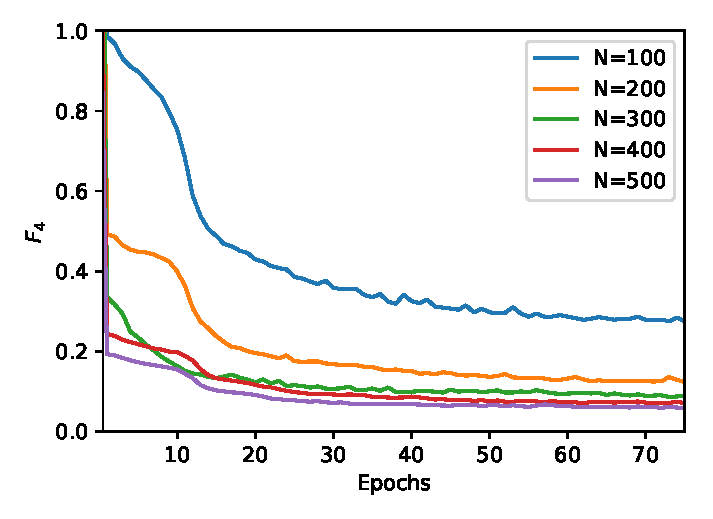
\includegraphics[width=\linewidth]{losses.pdf}
  %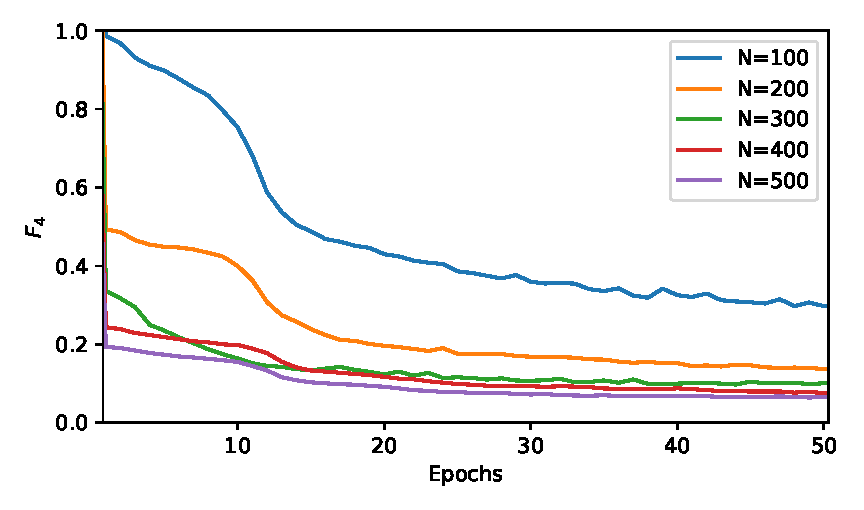
\includegraphics[width=0.85\linewidth]{losses2.pdf}
  
   However, the more important evaluation criterion is the sample-efficiency, i.e. how many samples ($N$) are required to achieve results comparable to EM if it were computationally tractable. Note that because samples are drawn without replacement, if $N$ approaches $2^C$, \emph{NVIF} becomes the EM-algorithm. Increasing $N$ is not expected to increase performance beyond a given point and the question arises when this point is reached.
   
  Figure \ref{f4} shows $F_4$ after convergence (300 epochs) for different numbers of samples $N$. One can see that the performance saturates quickly. The increase in performance from $400$ to $500$ is miniscule. Thus, by only exploring only about $1-2\%$ of the latent space, \emph{NVIF} achieves promising results.
  %\includegraphics[width=\linewidth]{inferred.png}
  \begin{figure}
      \centering
        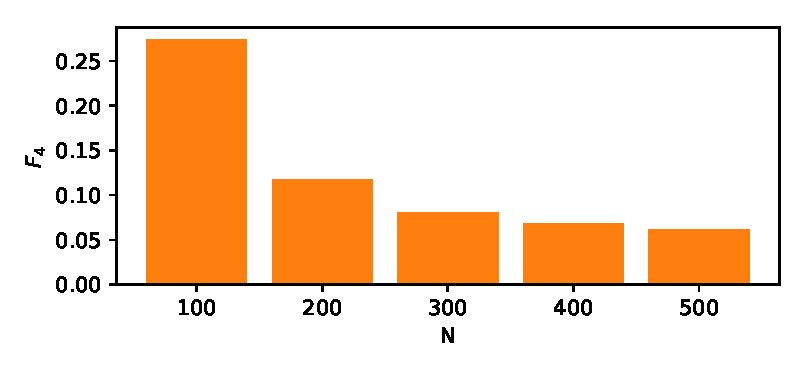
\includegraphics[width=0.8\linewidth]{nvif/losses3.pdf}
      \caption[NVIF: Performance as a function of number of samples.]{Performance measured by $F_4$ as a function of number of samples $N$ after convergence (300 epochs).}
      \label{f4}
  \end{figure}
  
   \begin{figure}[h!]
      \centering
        \includegraphics[width=0.8\linewidth]{nvif/inferred.png}
      \caption[NVIF: A comparison of the inferred components with ground truth appliances.]{A comparison of the inferred components with ground truth appliances.}
      \label{nvif:inferred}
  \end{figure}
  
%\noindent\rule[0.5ex]{\linewidth}{1pt}

\subsection{Conclusion}
To sum up, in this paper, an unbiased (given an appropriate choice of auxiliary distribution) algorithm for learning and inference in dynamical systems was introduced and evaluated in the context Non-Intrusive Load Monitoring. The algorithm was shown to be sample-efficient and even with a na\"ive model of NILM showed comparable results to existing algorithms. The introduced algorithm is general in nature and could in principle be applied to any dynamical system.